\mychapter{6}{Lesson 6}

\section{Computationally secure encryption}

\begin{question}
    How to define the concept of \textbf{computationally secure encryption} ?    
\end{question}

Find a task/scheme that is computationally hard for an attacker to break
(supposing the attacker is $ \poly{\lambda} $, we want a scheme which requires
an amount of time near ,as much as possible, to $superpoly(\lambda)$ to be
broken).

This scheme should have these properties:
\begin{itemize}
    \item \label{prop:owk} \textbf{one wayness} w.r.t. key (given $c=Enc(k,m)$,
        it should be hard to recover k) 
    \item \label{prop:owm} \textbf{one wayness}  w.r.t. message (given
        $c=Enc(k,m)$, hard to obtain the message)
    \item \label{prop:nol} no \textbf{information leakage} about the message
\end{itemize}.

Consider the experiment depicted in figure \ref{cryptogame:otindist} for the encryption scheme $\Pi = (Enc, Dec)$, where the adversary wins the game when the challenger outputs 1.

\begin{cryptogame}
    {otindist}
    {$\textsc{Game}_{\Pi, \textsf{A}}^{\textsc{ind}}(\lambda, b)$}
    {ind}

    \send{}{$m_0, m \in \M$}{}

    \receive{\shortstack[l]{
        $k \pickUAR \mathcal{K}$ \\
        $b \pickUAR \{0, 1\}$ \\
        $c \pickUAR Enc(k, m_b)$ }}
    {$c$}{}

    \cseqdelay

    \send{}{$b'$}{\textsc{Output 1 iff} $b = b'$}
    
\end{cryptogame}

\begin{definition}
    $\Pi$ is said to be computationally \textbf{one time secure} iff:
    \[
        \textsc{Game}_{\Pi, \textsf{A}}^{\textsc{ind}}(\lambda, 0) \compindist \textsc{Game}_{\Pi, \textsf{A}}^{\textsc{ind}}(\lambda, 1)
        \footnote{$\textsc{Game}_{\Pi, \textsf{A}}^{\textsc{ind}}$ refers to the indistinguishability of the messages sent by \textsf{A} during the game}
    \]  
    or, alternatively $\forall\; \textsc{ppt}\; \textsf{A}$:
    \[
        \lvert \Pr[\textsc{Game}_{\Pi, \textsf{A}}^{\textsc{ind}}(\lambda, 0) = 1] - \Pr[\textsc{Game}_{\Pi, \textsf{A}}^{\textsc{ind}}(\lambda, 1) = 1] \rvert \in \negl{\lambda}
    \]
\end{definition}

This last definition is compliant with the three properties exposed beforehand. In particular, if a scheme is \textbf{one time secure}, then it has each one of these 3 properties:

\todo{TO BE REVIEWED}

\begin{itemize}
    \item \textbf{compliance with point 1}: suppose point 1 is not valid, and $k$ is not hard to discover for \textsf{A}. Then \textsf{A} is able to perfectly distinguish $m$ and $m_{0}$ every time, therefore the scheme cannot be one time secure;
    \item \textbf{compliance with point 2}: suppose point 2 is not valid, and then the encrypted message can be easily discovered by \textsf{A}. Then, as before, \textsf{A} can win every game with $\Pr[1]$, so the scheme couldn't be one time secure;
    \item \textbf{compliance with point 3}: suppose point 3 is not valid, and some information about $m$ is leaked in $c$, for example the first bit of $c$ is the same bit of $m$. \textsf{A} could forge $m_0 = m$ such that they have the same bits but just the first is different. When \textsf{A} obtains $c$, he can look at the first bit and distinguish which was the message encrypted. Thus, the scheme wouldn't be one time secure.
\end{itemize}

What is not \textbf{two time secure}? Here is an apparently safe scheme, $\Pi_{\xor}$, where $G : \{0, 1\}^\lambda \to \{0, 1\}^l$ is a \prg:

\begin{itemize}
    \item $k \pickUAR \{0, 1\}^{\lambda} = \K$
    \item $Enc(k, m) = G(k) \xor m$, $m \in \{0, 1\}^{l}$
    \item $Dec(k, c) = c \xor G(k) = m$
\end{itemize}

To prove that $\Pi_{\xor}$ is not \textbf{two time secure}, assume an adversary \textsf{A} knows the pair $(\bar{m}, \bar{c} = G(k) \xor \bar{m})$. Then, given any ciphertext $c = G(k) \xor m$, where $m$ is unknown, \textsf{A} can efficiently compute the following: 
\[
    \bar{c} = G(k) \xor m = c \xor m \xor \bar{m} \Rightarrow c \xor \bar{c} = m \xor \bar{m} 
\]
and thus, by XORing the result with $\bar{m}$, obtain the entire unknown message\footnote{This example models a technique called ``Chosen Plaintext Attack'', which will be discussed in depth later}. Nevertheless, this scheme is still \textbf{one time secure}:

\begin{theorem}
    If $G$ is a \prg, then $\Pi_{\xor}$ is computationally \textbf{one time secure}
\end{theorem}

\begin{proof}
    We need to show that, $\forall\; \textsc{ppt}\; \textsf{A}$:
    \[
        \textsc{Game}_{\Pi_{\xor}, \textsf{A}}^{\textsc{ind}}(\lambda, 0) \compindist \textsc{Game}_{\Pi_{\xor}, \textsf{A}}^{\textsc{ind}}(\lambda, 1)
    \]

    Consider the hybrid game in figure \ref{cryptogame:xorothybrid}, where the original encryption routine is changed to use a random value instead of $G(k)$\footnote{The observant student may recognize that this modification yields exactly the One-Time Pad encryption scheme discussed in lesson 1}. Compare with the original \textbf{one time secure} definition in figure \ref{cryptogame:otindist} to observe that it perfectly matches.

    \begin{cryptogame}
        {xorothybrid}
        {$\textsc{Hyb}_{\Pi_{\xor}, \textsf{A}}(\lambda, b)$}
        {ind}

        \send{}{$m_0, m_1$}{}

        \receive{\shortstack[l]{
            $r \pickUAR \{0, 1\}^l$ \\
            $b \pickUAR \{0, 1\}$ \\
            $c = r \xor m_{b} $
        }}
        {$c$}{}

        \cseqdelay

        \send{}{$b'$}{\textsc{Output 1 iff} $b' = b$}
        
    \end{cryptogame}

    \begin{lemma}
        % AP181229: Lemma environment forces italics where it should not, this ugliness is a workaround
        \emph{\textrm{$\textsc{Hyb}_{\Pi_{\xor}, \textsf{A}}(\lambda, 0) \equiv \textsc{Hyb}_{\Pi_{\xor}, \textsf{A}}(\lambda, 1)$}}
    \end{lemma}

    \begin{proof}
    This is true because distribution of $c$ does not depend on $b \in \{0, 1\}$.
    \todo{Eh?}
    \end{proof}

    \begin{lemma}
        $ \forall b \in \{0,1\}, \textsc{Hyb}_{\Pi_{\xor}, \textsf{A}}(\lambda, b) \compindist \textsc{Game}_{\Pi_{\xor}, \textsf{A}}^{\textsc{ind}}(\lambda, b)$
    \end{lemma}

    \begin{proof}
        The proof proceeds by reduction as depicted in figure \ref{cryptoredux:xorotprg}, by assuming there exists a distinguisher $\textsf{D}^{\textsc{ind}}$ for $c = G(k) \xor m_{b}$ and $c = r \xor m_{b}$, and using it to break the \prg{} itself.

        \begin{cryptoredux}
            {xorotprg}
            {Reducing to breaking a \prg}
            {prg}
            {ind}

            \receive{\shortstack[l]{
                $x_0 \pickUAR G(U_\lambda)$ \\
                $x_1 \pickUAR U_l$ \\
                $b \pickUAR \{0, 1\}$
            }}
            {$x_b$}{}

            \return{}{$m_0, m_1$}{}

            \invoke{\shortstack[l]{
                $c = x_b \xor m_0$
            }}{$c$}{}

            \return{}{$b'$}{}

            \cseqdelay
            \send{$b'' = \begin{cases}
                0 &\textsc{iff } b'=0 \\
                1 &\textsc{else}
            \end{cases}$
            }{$b''$}{\textsc{Output 1 iff} $b'' = b$}

        \end{cryptoredux}

        Do observe that the adversary always encrypts $m_0$, but this game can be modified for $m_1$ by switching $b''$'s assignments without loss of generality; the crucial point is to see if the distinguisher guesses which message the adversary has encrypted:
        \begin{itemize}
            \item if $\textsf{D}^\textsc{ind}$ is wrong, then \textsf{A} can deduce with high probability that the value given by $\textsf{C}^\textsc{prg}$ is in fact truly random;
            \item if $\textsf{D}^\textsc{ind}$ is right, then \textsf{A} has a sensibly greater probability of having received a pseudorandom value from $\textsf{C}^\textsc{prg}$.
        \end{itemize} 

        Either way, by the existence of $\textsf{D}^\textsc{ind}$, \textsf{A} gains an edge in efficiently breaking a \prg{}, which is absurd.
    \end{proof}

    Finally, by the two above lemmas, the proof can be concluded by transitivity:
    \[
        \textsc{Game}_{\Pi_{\xor}, \textsf{A}}^{\textsc{ind}}(\lambda, 0) \compindist
        \textsc{Hyb}_{\Pi_{\xor}, \textsf{A}}(\lambda, 0) \equiv
        \textsc{Hyb}_{\Pi_{\xor}, \textsf{A}}(\lambda, 1) \compindist
        \textsc{Game}_{\Pi_{\xor}, \textsf{A}}^{\textsc{ind}}(\lambda, 1)
    \]

\end{proof}
 

\section{Pseudorandom functions}

\textsc{Prg}s are practically used as a stepping stone for building \emph{PseudoRandom Functions} (\prf), which in turn form the basis for most, if not all cryptographic schemes. Before introducing what a \prf{} formally is, a more intuitive definition of a \emph{truly random function} is given.

\begin{definition}
    A random function $R : \{0,1\}^{n} \to \{0,1\}^{l}$ is a function that, depending on what is known about its previous applications:

    \begin{itemize}
        \item if $x$ is ``fresh'' (in formal terms, $R$ has never been applied to $x$ beforehand), then a value $y$ is chosen \uar{} from $R$'s codomain, and it is permanently associated as the image of $x$ in $R$\footnote{this property is also called \emph{lazy sampling}};

        \item if $x$ is not fresh, then $R(x)$ is directly returned instead.
    \end{itemize}
\end{definition}

It sholud be noted that such functions occupy too much space, if we were to memorize it anywhere: supposing all the possible outputs of $R$ have been generated and stored as an array in memory, its size in bits will be $2^{n}l$.

\[  
    \color{black!50}%
    \overbracket[0.5pt][5pt]{{\thickspace}%
    \color{black}\printarray[4em]{0010...}\thickspace}^{l\textrm{ bits}}_{1}\thickspace%
    \overbracket[0.5pt][5pt]{{\thickspace}%
    \color{black}\printarray[4em]{1110...}\thickspace}^{l\textrm{ bits}}_{2}\thickspace%
    \overbracket[0.5pt][5pt]{{\thickspace}%
    \color{black}\printarray[4em]{0011...}\thickspace}^{l\textrm{ bits}}_{3}\thickspace%
    \color{black!25}\underbracket[0pt][5.5pt]{{\thickspace}%
    \printarray[2em]{...,...,...,...}\thickspace}_{}%
    \overbracket[0.5pt][5pt]{{\thickspace}%
    \color{black}\printarray[4em]{1111...}\thickspace}^{l\textrm{ bits}}_{2^{n}}\thickspace%
    \thickspace
\]

So we look for a kind of function which is ``random'', but does not require to be memorized as a whole map, while still being efficiently computable. This is where  pseudorandomness comes in: a function is deemed pseudorandom (a \prf) when it is (computationally) indistinguishable from a truly random one.

Usually, \prf{}s come as function families $F_k$, where $k$ is a key that identifies a single function inside the family itself\footnote{Those unfamiliar with the ``currying'' technique may see the key as an additional argument to pass to the ``main'' function $F$}.

With this in mind, let $\F=\{ F_{k}:\{0,1\}^{n(\lambda)} \to \{0,1\}^{l(\lambda)} \}_{k \in \{0,1\}^{\lambda}}$ be the \emph{keyed} function family that defines a \prf. Consider the two games in figure \ref{fig:prftwins}, each one involving respectively $\mathcal{F}$ and a random function $R$, where $\mathcal{R}=\{R : \{0, 1\}^{n} \to \{0, 1\}^{l}\}$, also written as $\mathcal{R}(\lambda, n, l)$ is the set of all random functions from $n$-bit strings to $l$-bit strings.

\begin{figure}[ht]
    \centering
    \sdinit{}
    \begin{tikzpicture}[scale=0.5]
        % Define symbols and names for the parties
        \sdbegin{}
        \newinst{A}{$ \A $}
        \newinst[2.3]{B}{$ C $} % Increase "5" to widen
        \mess{A}{$x$}{B}
        \node[anchor=west] at (mess to) {  };
        \postlevel
        \mess{B}{z}{A}
        \node[anchor=west] at (mess from) {\shortstack[l]{
            $k \pickUAR \{0,1\}^{\lambda}$ \\
            $z = F_{k}(x)$}};
        % Message from Bob to Alice, with computations by both sides
        \postlevel
        \mess{A}{$b'$}{B}
        \node[anchor=west] at (mess to) {  };
        \sdend{}
    \end{tikzpicture}
    \sdinit{}
    \begin{tikzpicture}[scale=.5]
        % Define symbols and names for the parties
        \sdbegin{}
        \newinst{A}{$ \A $}
        \newinst[2.3]{B}{$ C $} % Increase "5" to widen
        \mess{A}{$x$}{B}
        \node[anchor=west] at (mess to) {  };
        \postlevel
        \mess{B}{z}{A}
        \node[anchor=west] at (mess from) {\shortstack[l]{
            $R \pickUAR \R(\lambda, n, l)$ \\
            $z = R(x)$}};
        % Message from Bob to Alice, with computations by both sides
        \postlevel
        \mess{A}{$b'$}{B}
        \node[anchor=west] at (mess to) {  };
        \sdend{}
    \end{tikzpicture}

    \caption{$Real_{\F, \A}(\lambda)$ vs $Rand_{\R, \A}(\lambda)$}
    \label{fig:prftwins}
\end{figure}

$b' \in \{0,1\}$ is a convention and 1 is assigned to $Real$ or $Rand$; so in this game the adversary \textbf{recognizes} which machine he is talking with.

\begin{definition}
    $F_k$ is a \prf{} iff: 
    \[
        Real_{\F, \A}(\lambda) \compindist Rand_{\R, \A}(\lambda)
    \]
\end{definition}

\begin{exercise}
    Show that no \prg{} is secure against \textbf{unbounded attackers}.
\end{exercise}

\begin{exercise}
    Show the same as above, but for any \prf{} instead.
\end{exercise}

\pagebreak

\subsection{\textsc{Ggm}-tree}

In this section, it is described how to construct a \prf{} starting from a given \prg, using a technique devised form Goldreich, Goldwasser and Micali, called the \emph{\textsc{ggm}-tree}.

\begin{construction}
    Let $G : \{0, 1\}^{\lambda} \to \{0, 1\}^{2\lambda} $ be a \prg{} such that it doubles the length of its input, and splits ithe images in halves, effectively returning string couples: 
    \[
        G(k)=(G_{0}(k), G_{1}(k))
    \]

    Consider the \textsc{ggm}-tree depicted in figure \ref{fig:ggmtree}, which describes how $G$ will be used to craft a \prf. To lighten up the notation, a function composition $G_a(G_b(G_c(k)))$ will be contracted to $G_{abc}(k)$. So let $\F=\{F_{k} : \{0, 1\}^n \to \{0, 1\}^\lambda\}$ be a family of functions such that:
    \[
        F_k(r)=G_{r_{n}}(G_{r_{n-1}}( \dots G_{r_2}(G_{r_1}(k)) \dots ))
    \]

    \begin{figure}[htbp]
        \centering
        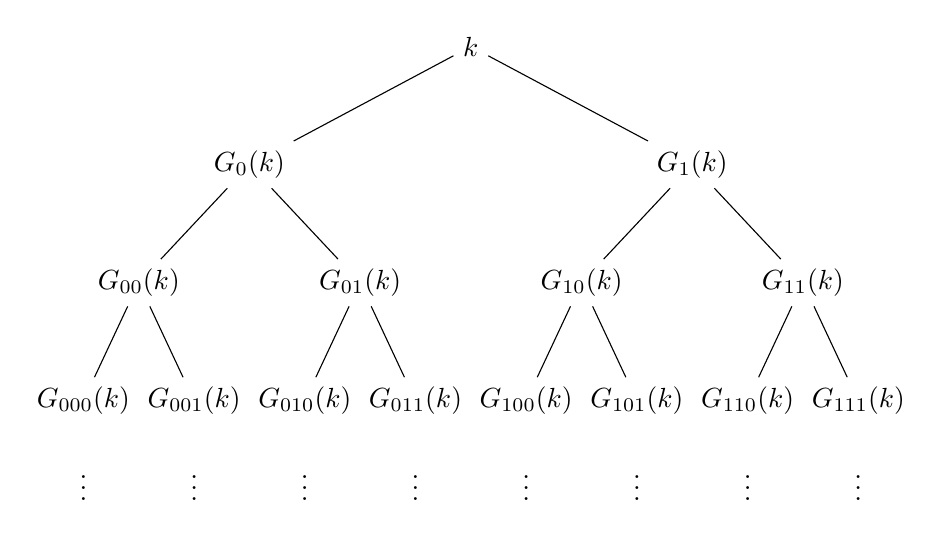
\begin{tikzpicture}[
            level 1/.style={sibling distance=16em},
            level 2/.style={sibling distance=8em},
            level 3/.style={sibling distance=4em}]

            \node{$k$}
                child{ node {$G_0(k)$}
                    child { node {$G_{00}(k)$}
                        child { node (a) {$G_{000}(k)$} node [below of = a] {$\vdots$}}
                        child { node (a) {$G_{001}(k)$} node [below of = a] {$\vdots$}}
                    }
                    child { node {$G_{01}(k)$}
                        child { node (a) {$G_{010}(k)$} node [below of = a] {$\vdots$}}
                        child { node (a) {$G_{011}(k)$} node [below of = a] {$\vdots$}}
                    }
                }
                child { node {$G_1(k)$}
                    child { node {$G_{10}(k)$}
                        child { node (a) {$G_{100}(k)$} node [below of = a] {$\vdots$}}
                        child { node (a) {$G_{101}(k)$} node [below of = a] {$\vdots$}}
                    }
                    child { node {$G_{11}(k)$}
                        child { node (a) {$G_{110}(k)$} node [below of = a] {$\vdots$}}
                        child { node (a) {$G_{111}(k)$} node [below of = a] {$\vdots$}}
                    }
                };
        \end{tikzpicture}
        \caption{The \textsc{ggm}-tree for $G$}
        \label{fig:ggmtree}
    \end{figure}

\end{construction}

An example, with a string value of $001$ for $r$ would evaluate as $F_k(001) = G_0(G_0(G_1(k)))$.

